\section{Технический проект}
\subsection{Общая характеристика организации решения задачи}

Необходимо спроектировать и разработать приложение, который должен способствовать популяризации ролевых игр.

Приложение представляет собой набор взаимосвязанных различных окон, которые сгруппированы по разделам, содержащие текстовую, графическую информацию. Приложение располагается на компьютере.

\subsection{Обоснование выбора технологии проектирования}

На сегодняшний день информационный рынок, поставляющий программные решения в выбранной сфере, предлагает множество продуктов, позволяющих достигнуть поставленной цели – разработки приложения.

\subsubsection{Описание используемых технологий и языков программирования}

В процессе разработки приложения используются программные средства и языки программирования. Каждое программное средство и каждый язык программирования применяется для круга задач, при решении которых они необходимы.

\subsubsection{Язык программирования Python}

Python –  высокоуровневый язык программирования общего назначения с динамической строгой типизацией и автоматическим управлением памятью, ориентированный на повышение производительности разработчика, читаемости кода и его качества, а также на обеспечение переносимости написанных на нём программ. Язык является полностью объектно-ориентированным в том плане, что всё является объектами. Необычной особенностью языка является выделение блоков кода отступами. Синтаксис ядра языка минималистичен, за счёт чего на практике редко возникает необходимость обращаться к документации. Сам же язык известен как интерпретируемый и используется в том числе для написания скриптов. Недостатками языка являются зачастую более низкая скорость работы и более высокое потребление памяти написанных на нём программ по сравнению с аналогичным кодом, написанным на компилируемых языках, таких как C или C++.

\subsubsection{Использование библиотеки Tkinter и реализация таймеров на Python}
	
\paragraph{Введение}
Библиотека Tkinter - это стандартная библиотека Python для создания графического пользовательского интерфейса (GUI). Она обладает широкими возможностями для создания разнообразных приложений с использованием различных виджетов, таких как кнопки, поля ввода, метки и многое другое.
	
\paragraph{Возможности Tkinter}
Вот некоторые из основных возможностей, предоставляемых библиотекой Tkinter:
	
\begin{itemize}
	\item Создание различных виджетов: кнопки, метки, поля ввода, списки и многое другое.
	\item Управление компоновкой виджетов с использованием менеджеров компоновки (например, grid, pack, place).
	\item Обработка событий, таких как щелчок мыши, нажатие клавиш и другие.
	\item Возможность создания различных диалоговых окон, таких как окна предупреждений, информационные окна и окна запроса.
	\item Поддержка многопоточности для обновления интерфейса из различных потоков выполнения.
\end{itemize}
	
\paragraph{Реализация таймеров на Python}
Для реализации таймеров на Python можно использовать модуль \texttt{time} или \texttt{threading}. Вот пример использования модуля \texttt{time} для создания простого таймера:
	
	import time
	
	def countdown(t):
	while t > 0:
	mins, secs = divmod(t, 60)
	timeformat = '{:02d}:{:02d}'.format(mins, secs)
	print(timeformat, end='\r')
	time.sleep(1)
	t -= 1
	print('Таймер завершен!')
	

	t = 10
	countdown(t)
	
Этот код создает простой обратный отсчет таймера с использованием функции \texttt{countdown}. Он выводит оставшееся время в формате ММ:СС и уменьшает его на 1 каждую секунду, используя функцию \texttt{time.sleep(1)}. Когда время истекает, выводится сообщение о завершении таймера.
	
\paragraph{Заключение}
Библиотека Tkinter предоставляет мощные инструменты для создания графических пользовательских интерфейсов на языке Python. Реализация таймеров на Python может быть достигнута с помощью модулей \texttt{time} или \texttt{threading}, в зависимости от конкретных требований приложения.

\subsection{Описание платформы для создания RPG игр}
Клиент создает модуль содержащий методы модуля RPGGame, например bggame. В этом модуле мы создаем мир игры, с помощью new\_actor. Мы можем вызывать их много раз с разными параметрами, или загрузить параметры для этих функций из файла. После чего у нас есть персонажи и предметы. Мир также состоит из зон (Area). Каждая зона включает в себя графику, персонажи и предметы и сценарии взаимодействия. Исключение составляет команда PC, которая может перемещаться из зоны в зону (это мы программируем у клиента). Команду мы тоже определяем стартовую и впоследствии можем менять (add\_actor\_to\_team, remove\_actor\_from\_team). Каждому персонажу и объекту может соответствовать пользовательский сценарий (он активируется при нажатии мышкой на объект). Сценарий может включать диалог, взятие предмета, добавление персонажа в команду, квест и т.д.
Зона тоже может содержать сценарий, который запускается когда команда попадает в зону.
Клиентский класс (BGGame) также содержит глобальные переменные, определяющие ситуации в игре (например квесты). Локальные переменные могут быть в зоне.

Как программируются зоны. Если нужны локальные переменные (состояние локальных событий), то тогда нужно создавать класс своей зоны как наследник от Area. Или же просто использовать класс Area. Добавляем зону в игру new\_area(name, area). Переключаем зону - set\_area(name). Глобальные сценарии находятся в классе игры (BGGame), мы подключаем их как :
Area.set\_enter\_script(script)
В зону мы добавляем персонажей и предметы как add\_object(x,y, obj) - z не нужно, так как слой можно определить по y координате.
В конкретную зону мы добавляем сценарий для взаимодействия как: Game.game.start\_script(script, name)
Как происходит переход команды между зонами.
В зоне определяем объект дверь, по клику мыши она может открываться и закрываться (меняется состояние объекта). Назначаем сценарий walk\_script(script), который срабатывает когда кто-то из команды пересекает объект. В этом сценарии мы меняем зону на нужную (set\_area), и устанавливаем команду в нужную позицию (set\_team). В другой зоне делается аналогично, только переход и позиция будут другими.
Сценарии - это потоки которые запускаются параллельно (метод RPGGame.start\_script(script)). Сценарий может быть остановлен (stop\_script(name)).
Таким образом, мир будет интерактивным.
Как связано окно и графика с игрой. В окне мы делаем таймер, который вызывает метод update нашей игры (BGGame). Этот метод выполняет все действия объектов в игре за 1 кадр времени.
Также в таймере вызываем Graphics.update(), который обновляет графику игры.
Все объекты (Actor, Item) должны иметь состояния (как минимум одно). Каждое состояние связано с спрайтом (или анимацией). То есть переключение состояния меняет графику объекта.

А вообще сценарии и глобальные переменные могут быть без классов, а просто в модулях, так проще, чтобы к ним был доступ из всех комнат. Тогда и функции движка должны быть доступны везде (то есть во всех сценариях). Например делаем модуль руины (ruins):
import random
from math import sqrt
import time
from rpg.area import *
from rpg.sprite import *
from rpg.rectangle import *
from rpg.game import Game
from rpg.portal import Portal

class Ruins(Area):
def \_\_init\_\_(self):
'''
Класс игровой зоны Ruins

'''
super().\_\_init\_\_()
self.add\_sprite(Sprite('images/fon3.png'), 590, 400, 0)
self.add\_rect(Rectangle(x=0, y=0, width=Sprite('images/fon3.png').image.width(), height=Sprite('images/fon3.png').image.height()))
from grunt import Grunt
self.grunt = Grunt(0,0,0)
from footman import Footman
self.footman = Footman(0,0,0)
self.add\_object(self.footman, 120, 120, 1)
self.add\_object(self.grunt, 500, 185, 1)
p = Portal(400, 400, 200, 200, 'Village', 480, 100)
self.add\_object(p, p.pos\_x, p.pos\_y, 100)
Game.game.start\_script(self.ai, "ai", self.grunt)
Game.game.start\_script(self.walk\_two, "footman", 50, 50)


def walk(self, step\_x, step\_y, actor):
'''
Сценарий для движения бугая

:param step\_x: шаг движения x
:param step\_y: шаг движения y
'''
if actor.hp <= 0:
Game.game.stop\_script("grunt")
new\_x = 200
new\_y = 200
actor.is\_attack = False
direction = random.choice(["up", "down", "left", "right"])
if direction == "up":
new\_y -= step\_y
new\_x = step\_x
elif direction == "down":
new\_y += step\_y
new\_x = step\_x
elif direction == "left":
new\_y = step\_y
new\_x -= step\_x
elif direction == "right":
new\_y = step\_y
new\_x += step\_x

actor.search\_position(new\_x, new\_y)

time.sleep(2)

модуль bggame:
from ruins import *
import time
import random

class BaldursGame(Game):
def \_\_init\_\_(self, canvas, window, **params):
'''
Класс конкретной игры для демонстрации

:param canvas: класс графической системы
:param window: окно на которое будет выводится игра
'''
super().\_\_init\_\_(canvas, window, **params)
from mage import Mage
self.add\_pc\_to\_team(Mage(0, 0, 0))
self.new\_area('Ruins', Ruins())
self.set\_area('Ruins')
self.set\_team(500, 300, 100)
self.timer()

\subsubsection{Пример клиентского кода игры}
\paragraph{Cоздание классов персонажей/предметов}
Клиент создает модуль содержащий методы модуля RPGGame, например BaldursGateGame. В этом модуле клиент создаем мир игры, с помощью new\_actor. 

модуль bggame:
from ruins import *
import time
import random

class BaldursGame(Game):
def \_\_init\_\_(self, canvas, window, **params):
'''
Класс конкретной игры для демонстрации

:param canvas: класс графической системы
:param window: окно на которое будет выводится игра
'''
super().\_\_init\_\_(canvas, window, **params)
from mage import Mage
self.add\_pc\_to\_team(Mage(0, 0, 0))
self.new\_area('Ruins', Ruins())
self.set\_area('Ruins')
self.set\_team(500, 300, 100)
self.timer()

\paragraph{Задание правил атаки}
Пользователь создаёт класс ADnDActor, наследник от класса Actor в своём модуле bggame, в нём он прописывает свои правила по которым происходит атака. То есть Actor.attack(self, actor), где actor - кого атакуют.
Пример:

модуль adnd\_actor:
from math import sqrt
from rpg.actor import Actor
from rpg.animation import Animation
import rpg.game
import time

class Adnd\_actor(Actor):

ATTACK\_RANGE = 50

def \_\_init\_\_(self, x, y, z, **params):
'''
Класс Adnd\_actor содержащий основные механики взаимодействия с другими персонажами

:param x: координата x
:param y: координата y
:param z: координата z
'''
super().\_\_init\_\_(x, y, z, **params)
self.on\_click = self.click

def click(self):
'''
вызывается при клике на персонажа

'''
pc = rpg.game.Game.game.team\_of\_pc[0]
if pc == self:
return
dx = pc.pos\_x - self.pos\_x
dy = pc.pos\_y - self.pos\_y
dist = sqrt(dx * dx + dy * dy)
if dist <= self.ATTACK\_RANGE:
pc.is\_attack = True
pc.attack(self)
time.sleep(0.125)
if self.hp <=0:
pc.is\_attack = False

def attack(self, actor):
'''
совершает атаку по actor

:param actor: персонаж, которого атакуют
'''
actor.hp -= self.damage
def update(self):
'''
обновляет состояние персонажа

'''
super().update()
if self.hp <= 0:
self.stop\_move()
self.set\_state('death')


\paragraph{Создание зон, заполнение их персонажами/объектами}
Мир также состоит из зон (Area). Каждая зона включает в себя графику, персонажи и предметы и сценарии взаимодействия. Исключение составляет команда PC, которая может перемещаться из зоны в зону (это мы программируем у клиента). Как программируются зоны. Если нужны локальные переменные (состояние локальных событий), то тогда нужно создавать класс своей зоны как наследник от Area. Или же просто использовать класс Area. Добавляем зону в игру new\_area(name, area). Переключаем зону - set\_area(name). Так же требуется задать область движения, её проще сделать как совокупность прямоугольников, за которые персонажи не могут выйти. Эти прямоугольники должны касаться друг друга, но не пересекаться. Тогда алгоритм проверки выхода несложный: выход за пределы области только тогда, когда прямоугольник персонажа пересек сторону (одну или две) одного из прямоугольников области, эта сторона не является касательной.

import random
from math import sqrt
import time
from rpg.area import *
from rpg.sprite import *
from rpg.rectangle import *
from rpg.game import Game
from rpg.portal import Portal

class Ruins(Area):
def \_\_init\_\_(self):
'''
Класс игровой зоны Ruins

'''
super().\_\_init\_\_()
self.add\_sprite(Sprite('images/fon3.png'), 590, 400, 0)
self.add\_rect(Rectangle(x=0, y=0, width=Sprite('images/fon3.png').image.width(), height=Sprite('images/fon3.png').image.height()))
from grunt import Grunt
self.grunt = Grunt(0,0,0)
from footman import Footman
self.footman = Footman(0,0,0)
self.add\_object(self.footman, 120, 120, 1)
self.add\_object(self.grunt, 500, 185, 1)
p = Portal(400, 400, 200, 200, 'Village', 480, 100)
self.add\_object(p, p.pos\_x, p.pos\_y, 100)
Game.game.start\_script(self.ai, "ai", self.grunt)
Game.game.start\_script(self.walk\_two, "footman", 50, 50)


def walk(self, step\_x, step\_y, actor):
'''
Сценарий для движения бугая

:param step\_x: шаг движения x
:param step\_y: шаг движения y
'''
if actor.hp <= 0:
Game.game.stop\_script("grunt")
new\_x = 200
new\_y = 200
actor.is\_attack = False
direction = random.choice(["up", "down", "left", "right"])
if direction == "up":
new\_y -= step\_y
new\_x = step\_x
elif direction == "down":
new\_y += step\_y
new\_x = step\_x
elif direction == "left":
new\_y = step\_y
new\_x -= step\_x
elif direction == "right":
new\_y = step\_y
new\_x += step\_x

actor.search\_position(new\_x, new\_y)

time.sleep(2)

модуль bggame:
from ruins import *
import time
import random

\paragraph{Пример сценариев: переход между зонами}
Глобальные сценарии находятся в классе игры (BGGame), мы подключаем их как :
Area.set\_enter\_script(script)
Как происходит переход команды между зонами.
В зоне определяем объект портал, по клику мыши когда персонаж заходит внутрь портала срабатывает self.actor\_in(self, actor). При создании портала, мы указываем кудаи в какую зону разместить команду персонажей.

from rpg.object import Object
from rpg.game import Game
from rpg.rectangle import Rectangle

class Portal(Object):
def \_\_init\_\_(self, x, y, width, height, area, team\_x, team\_y):
''' 
Создает портал в новую зону

:param x: координата x портала
:param y: координата y портала
:param width: ширина портала
:param height: высота портала
:param area: имя зоны куда будет переход
:param team\_x: местоположение команды в новой зоне
:param team\_y: местоположение команды в новой зоне
'''
self.states = None
self.sprite = None
self.category = 'portal'
super().\_\_init\_\_(x, y, 0)
self.rectangle = Rectangle(x, y, width, height)
self.area = area
self.team\_x = team\_x
self.team\_y = team\_y
self.visible = False

def actor\_in(self, actor):
'''
Проверяет находится ли персонаж внутри портала

:param actor: проверяемый персонаж
'''
if actor.category == "pc":
Game.game.set\_area(self.area)
Game.game.set\_team(self.team\_x, self.team\_y, 100)
actor.stop\_move()

модуль ruins
import random
from math import sqrt
import time
from rpg.area import *
from rpg.sprite import *
from rpg.rectangle import *
from rpg.game import Game
from rpg.portal import Portal

class Ruins(Area):
def \_\_init\_\_(self):
'''
Класс игровой зоны Ruins

'''
super().\_\_init\_\_()
self.add\_sprite(Sprite('images/fon3.png'), 590, 400, 0)
self.add\_rect(Rectangle(x=0, y=0, width=Sprite('images/fon3.png').image.width(), height=Sprite('images/fon3.png').image.height()))
from grunt import Grunt
self.grunt = Grunt(0,0,0)
from footman import Footman
self.footman = Footman(0,0,0)
self.add\_object(self.footman, 120, 120, 1)
self.add\_object(self.grunt, 500, 185, 1)
p = Portal(400, 400, 200, 200, 'Village', 480, 100)

\paragraph{Как будет идти бой}
Бой будет совершаться с помощью сценариев. У класса Adnd\_actor есть метод attack(self, actor), который уменьшает текущее количество здоровья у actor. В модуле game существуют методы start\_script(script, name), stop\_script(name). С помощь сценариев возможно запускать параллельные потоки. В конкретную зону будет добавляться сценарий 'ai', в который передаётся конкретный персонаж. В этом сценарии указывается поведение противника, Что он должен сближаться с персонажем игрока, и когда расстояние до атаки будет достаточным, чтобы её совершить, будет вызван метод actor.attack. Для того, чтобы пользователь мог атаковать персонажа, у каждого экземпляра класса adnd\_actor есть метод click(self), который вызывает проверку условия, если персонаж близко к персонажу игрока, хранящемуся в rpg.game.Game.team\_of\_pc, то вызвать у pc=rpg.game.Game.team\_of\_pc[0], attack(self)/
Пример:
модуль adnd\_actor:
from math import sqrt
from rpg.actor import Actor
from rpg.animation import Animation
import rpg.game
import time

class Adnd\_actor(Actor):

ATTACK\_RANGE = 50

def \_\_init\_\_(self, x, y, z, **params):
'''
Класс Adnd\_actor содержащий основные механики взаимодействия с другими персонажами

:param x: координата x
:param y: координата y
:param z: координата z
'''
super().\_\_init\_\_(x, y, z, **params)
self.on\_click = self.click

def click(self):
'''
вызывается при клике на персонажа

'''
pc = rpg.game.Game.game.team\_of\_pc[0]
if pc == self:
return
dx = pc.pos\_x - self.pos\_x
dy = pc.pos\_y - self.pos\_y
dist = sqrt(dx * dx + dy * dy)
if dist <= self.ATTACK\_RANGE:
pc.is\_attack = True
pc.attack(self)
time.sleep(0.125)
if self.hp <=0:
pc.is\_attack = False

def attack(self, actor):
'''
совершает атаку по actor

:param actor: персонаж, которого атакуют
'''
actor.hp -= self.damage
def update(self):
'''
обновляет состояние персонажа

'''
super().update()
if self.hp <= 0:
self.stop\_move()
self.set\_state('death')

модуль ruins
import random
from math import sqrt
import time
from rpg.area import *
from rpg.sprite import *
from rpg.rectangle import *
from rpg.game import Game
from rpg.portal import Portal

class Ruins(Area):
def \_\_init\_\_(self):
'''
Класс игровой зоны Ruins

'''
super().\_\_init\_\_()
self.add\_sprite(Sprite('images/fon3.png'), 590, 400, 0)
self.add\_rect(Rectangle(x=0, y=0, width=Sprite('images/fon3.png').image.width(), height=Sprite('images/fon3.png').image.height()))
from grunt import Grunt
self.grunt = Grunt(0,0,0)
from footman import Footman
self.footman = Footman(0,0,0)
self.add\_object(self.footman, 120, 120, 1)
self.add\_object(self.grunt, 500, 185, 1)
p = Portal(400, 400, 200, 200, 'Village', 480, 100)
self.add\_object(p, p.pos\_x, p.pos\_y, 100)
Game.game.start\_script(self.ai, "ai", self.grunt)
Game.game.start\_script(self.walk\_two, "footman", 50, 50)


def walk(self, step\_x, step\_y, actor):
'''
Сценарий для движения бугая

:param step\_x: шаг движения x
:param step\_y: шаг движения y
'''
if actor.hp <= 0:
Game.game.stop\_script("grunt")
new\_x = 200
new\_y = 200
actor.is\_attack = False
direction = random.choice(["up", "down", "left", "right"])
if direction == "up":
new\_y -= step\_y
new\_x = step\_x
elif direction == "down":
new\_y += step\_y
new\_x = step\_x
elif direction == "left":
new\_y = step\_y
new\_x -= step\_x
elif direction == "right":
new\_y = step\_y
new\_x += step\_x

actor.search\_position(new\_x, new\_y)

def ai(self, actor):
'''
скрипт противников

:param step\_x: размер шага x до персонажа игрока
:param step\_y: размер шага x до персонажа игрока
:param actor: персонаж противник
'''
if actor.hp <= 0:
Game.game.stop\_script("ai")
import rpg.game
pc = rpg.game.Game.game.team\_of\_pc[0]
new\_x = pc.pos\_x
new\_y = pc.pos\_y

actor.search\_position(new\_x, new\_y)
dx = pc.pos\_x - actor.pos\_x
dy = pc.pos\_y - actor.pos\_y
dist = sqrt(dx * dx + dy * dy)
if dist <= actor.ATTACK\_RANGE:
actor.is\_attack = True
actor.attack(pc)
time.sleep(1)
if pc.hp <=0:
actor.update()
Game.game.stop\_script("ai")
Game.game.start\_script(self.walk, "grunt", 50, 50, actor)

else:
actor.is\_attack = False
time.sleep(2)

\paragraph{Соединение движка и окон tkinter}
Модуль graphics содержит в себе библиотеку tkinter . Класс Graphics внутри модуля является наследником tk.Canvas. Этот класс взаимодействует с окном root = tk.TK() в программном модуле пользователя. Модуль sprite тоже взаимодействует с tkinter. Изображение для спрайта берётся с помощью метода tk.PhotoImage(file=name)

модуль sprite

import tkinter as tk
class Sprite:

def \_\_init\_\_(self, image):
'''
Класс спрайта для работы с изображениями на Canvas

:param image: адресс изображения который
'''
self.image = tk.PhotoImage(file=image)
self.tag = None
self.x = 0
self.y = 0
self.z = 0

def set\_tag(self, tag):
'''
Устанавливает тег спрайта

:param tag: тег спрайта
'''
self.tag = tag

def set\_z(self, z):
'''
Устанавливает z-координату спрайта

:param z: координата z
'''
self.z = z

def get\_tag(self):
'''
Возвращает тег спрайта

'''
return self.tag

def set\_coords(self, new\_x, new\_y):
'''
Обновляет координаты спрайта

:param new\_x: координата x
:param new\_y: координата y
'''
if self.tag:
self.x = new\_x
self.y = new\_y
def update(self):
'''
Обновляет анимацию спрайта

'''
pass

модуль graphics

import tkinter as tk

class Graphics(tk.Canvas):
canvas = None
def \_\_init\_\_(self, master, **kwargs):
'''
Класс с методами для работы со спрайтами

'''
super().\_\_init\_\_(master, **kwargs)
self.sprites = []
Graphics.canvas = self

def add\_sprite(self, sprite, x, y, z, **kwargs):
'''
Добавляет спрайт на Canvas

:param sprite: спрайт
:param x: координата x
:param y: координата y
:param z: координата z
:param kwargs: параметры относящиеся к конкретному изображению в tkinter
'''
tag = self.create\_image(x, y, image=sprite.image, anchor='center', **kwargs)
sprite.set\_tag(tag)
sprite.set\_z(z)
sprite.x = x
sprite.y = y
self.sprites.append(sprite)
self.sprites.sort(key=lambda sprite: sprite.z)

def update(self):
'''
Перерисовывает все спрайты

'''
for sprite in self.sprites:
sprite.update()
self.tag\_raise(sprite.get\_tag())
self.coords(sprite.get\_tag(), sprite.x, sprite.y)
self.itemconfig(sprite.get\_tag(), image=sprite.image)


def change\_sprite(self, sprite, new\_sprite):
'''
Меняет  спрайт на новый.

:param sprite: экземпляр спрайта
:param new\_sprite: новый спрайт
'''
old\_sprite\_pos = None
for i, s in enumerate(self.sprites):
if s.get\_tag() == sprite.get\_tag():
old\_sprite\_pos = i
break

if old\_sprite\_pos is not None:
old\_tag = sprite.get\_tag()

self.sprites[old\_sprite\_pos] = new\_sprite
new\_sprite.set\_tag(old\_tag)

new\_sprite.set\_tag(old\_tag)
new\_sprite.set\_z(sprite.z)

self.tag\_raise(old\_tag)
self.coords(old\_tag, sprite.x, sprite.y)
self.itemconfig(old\_tag, image=new\_sprite.image)

def delete\_sprite(self, sprite):
'''
Удаляет спрайт с Canvas.

:param sprite: экземпляр спрайта
:return:
'''
self.delete(sprite.get\_tag())
self.sprites.remove(sprite)

def clear\_all(self):
'''
Удаляет все спрайты с Canvas

'''
for sprite in self.sprites:
self.delete(sprite.get\_tag())
self.sprites.clear()

модуль baldursgame '''пользовательский модуль'''

from ruins import *
from village import *
import time
import random

class BaldursGame(Game):
def \_\_init\_\_(self, canvas, window, **params):
'''
Класс конкретной игры для демонстрации

:param canvas: класс графической системы
:param window: окно на которое будет выводится игра
'''
super().\_\_init\_\_(canvas, window, **params)
from mage import Mage
self.add\_pc\_to\_team(Mage(0, 0, 0))
self.new\_area('Ruins', Ruins())
self.new\_area('Village', Village())
self.set\_area('Ruins')
self.set\_team(500, 300, 100)
self.timer()

модуль main
from bggame import *

root = tk.Tk()
root.geometry('1500x1500')

exit\_button = tk.Button(root, text="Exit", fg="red", command=root.destroy)
canvas = Graphics(root, width=1500, height=1500)
Graphics.canvas = canvas

BaldursGame(canvas, root)

canvas.place(height = 1500, width =1500)
BaldursGame.timer

root.mainloop()

\subsection{Архитектура платформы для создания ролевых игр}
\subsubsection{Диаграмма компонентов классов}
Диаграмма компонентов описывает особенности физического представления разрабатываемой системы. Она позволяет определить архитектуру системы, установив зависимости между программными компонентами, в роли которых может выступать как исходный, так и исполняемый код. Основными графическими элементами диаграммы компонентов являются компоненты, интерфейсы, а также зависимости между ними. На рисунке \ref{diagram.eps:image} изображена диаграмма компонентов для проектируемой системы. Она включает в себя основной класс платформы игры Game и производные от него классы, класс Object с наследниками и их параметрами (полями и методами).
\begin{figure}[ht]
	\center{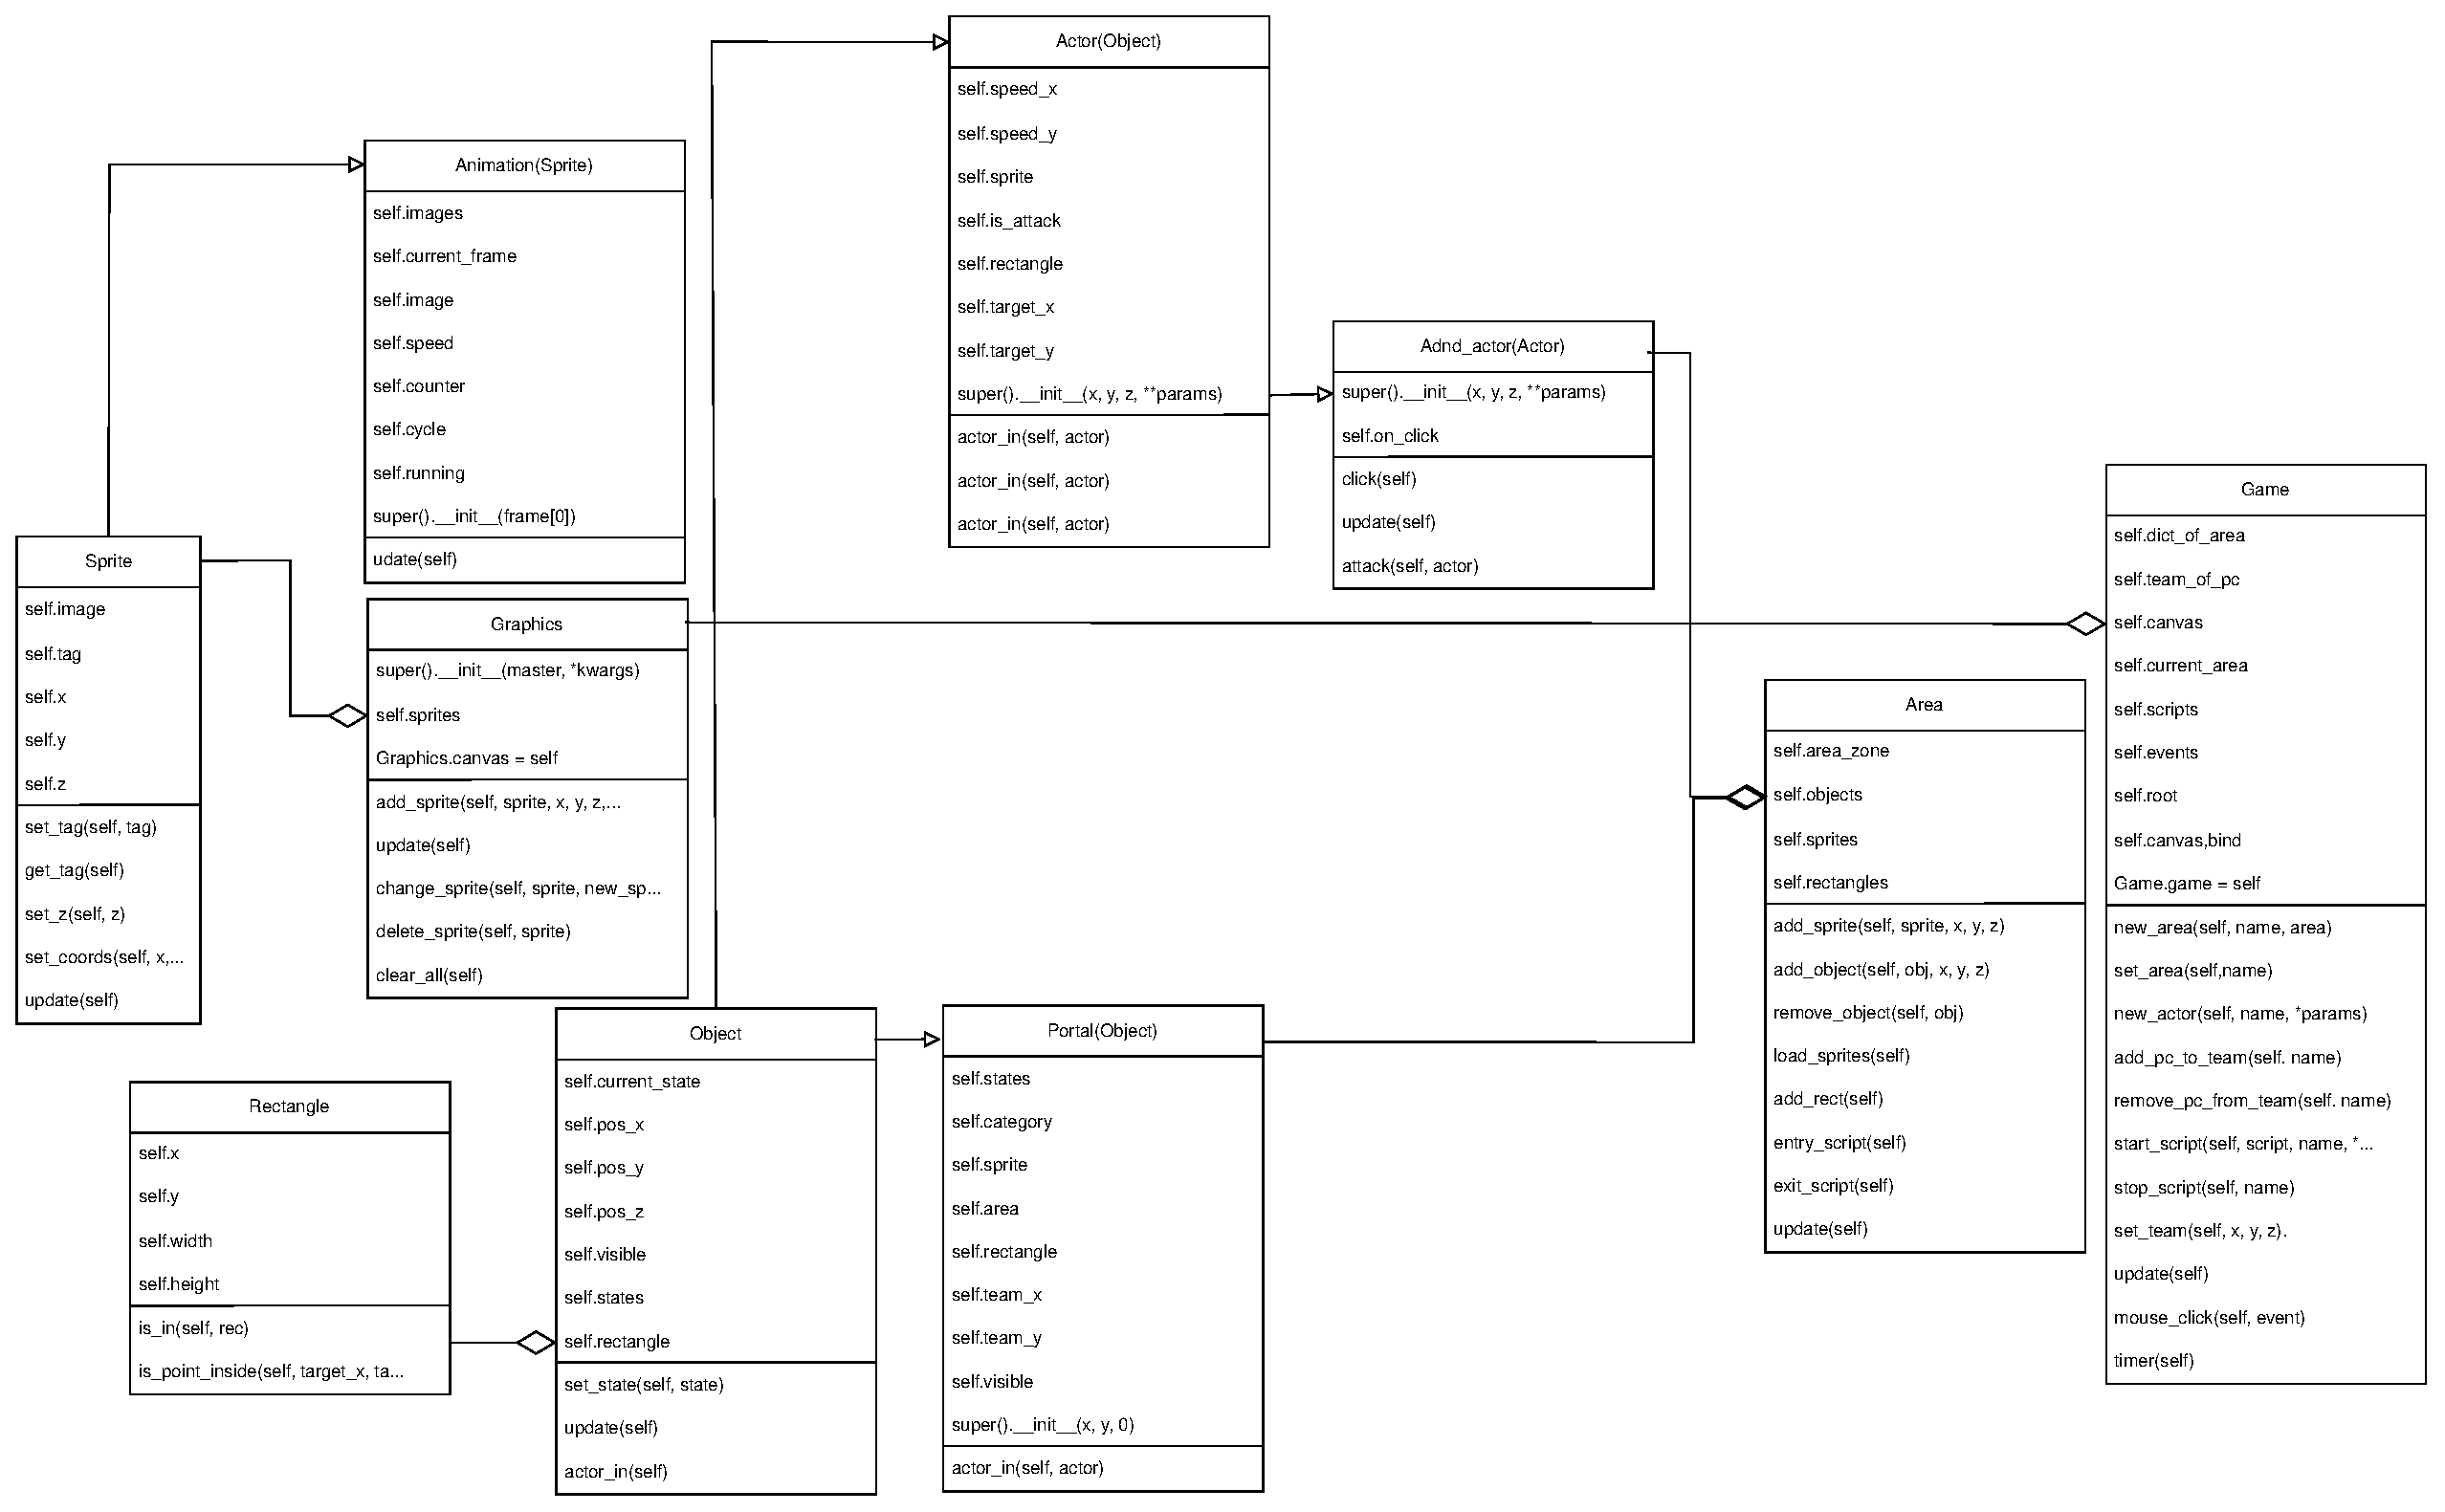
\includegraphics[width=1\linewidth]{diagram}}
	\caption{Диаграмма компонентов}
	\label{diagram:image}
\end{figure}
\paragraph{Описание классов}
\begin{enumerate}
	\item[Graphics] - класс, управляющий спрайтами. Содержит в себе:
	\begin{itemize}
		\item self.sprites - список спрайтов;
		\item add\_sprite(self, sprite x, y, z, image) - добавляет в список спрайт, сохраняет координаты;
		\item change\_sprite(self, sprite new\_sprite) - меняет местами спрайты в списке.
		\item delete\_sprite(self, sprite) - удаляет спрайт из списка.
		\item clear\_all(self) - очищает список спрайтов.
		\item update(self) - добавляет все спрайты из списка на форму.
	\end{itemize}
	\item[Sprite] - класс, хранящий в себе изображение игровых объектов image.
	\begin{itemize}
		\item self.x - координата x.
		\item self.y - координата y.
		\item self.z - координата z.
		\item self.tag - уникальный номер спрайта.
		\item self.image - изображение.
		\item set\_tag(self, tag) - устанавливает tag спрайту.
		\item get\_tag(self) - возвращает tag спрайта.
		\item set\_z(self, z) - устанавливает z координату.
		\item set\_coords(self, new\_x, new\_y) - устанавливает новые координаты.
		\item update(self) - ничего не делает.
	\end{itemize}
	\item[Animation] - класс, хранящий в себе список изображений игровых объектов image. Потомок класса Sprite.
	\begin{itemize}
		\item self.current\_frame - текущий кадр.
		\item self.images  - Загрузка всех кадров анимации.
		\item self.image - Установка начального изображения.
		\item self.speed - скорость анимации.
		\item self.counter - счётчик кадров.
		\item self.cycle - проверка на то что должна ли быть анимация циклично или нет.
		\item self.running - проверка проигрывается ли сейчас анимация.
		\item update(self) - обновляет кадр в анимации.
	\end{itemize}
	\item[Rectangle] - абстрактный класс прямоугольника.
	\begin{itemize}
		\item self.pos\_x - координата x.
		\item self.pos\_y - координата y.
		\item self.width - ширина.
		\item self.height - высота.
		\item is\_in(self, rect) - функция проверки нахождения одного прямоугольника в другом.
		\item is\_point\_inside(self, target\_x, target\_y) - функция проверки точки в пределах прямоугольника.
	\end{itemize}
	\item[Object] - класс, от которого наследуются классы Adnd\_Actor, Actor, Portal.
	\begin{itemize}
		\item self.pos\_x - координата x.
		\item self.pos\_y - координата y.
		\item self.pos\_z - координата z.
		\item self.current\_state - текущее состояние.
		\item self.visible - видимость портала.
		\item self.on\_click - функция клика по объекту.
		\item self.rectangle - прямоугольник объекта.
		\item set\_state(self, state\_name) -устанавливает состояние.
		\item actor\_in(self, actor) - ничего не делает.
		\item update(self) - ничего не делает.
	\end{itemize}
	\item[Portal] - класс объекта для перехода между зонами. Потомок класса Object.
	\begin{itemize}
		\item self.states - состояние портала.
		\item self.sprite - спрайт портала.
		\item self.category - категория.
		\item self.rectangle = - прямоугольник портала.
		\item self.area - зона в которую ведёт портал.
		\item self.team\_x - координата x в  которую нужно разместить команду.
		\item self.team\_y - координата y в  которую нужно разместить команду.
		\item self.visible - видимость портала.
		\item actor\_in(actor) - события, которые произойдут, когда персонаж окажется внутри прямоугольника портала.
	\end{itemize}
	\item[Actor] - класс персонажа, содержащий внутри себя основные поля и методы для перемещения по рабочему окну.
	\begin{itemize}
		\item self.sprite - спрайт персонажа.
		\item self.speed\_x - значение скорости x.
		\item self.speed\_y - значение скорости y.
		\item self.target\_x - координата x в которую должен прийти персонаж.
		\item self.target\_y - координата y в которую должен прийти персонаж.
		\item self.rectangle - прямоугольник персонажа.
		\item self.is\_attack - атакует ли сейчас персонаж.
		\item update(self) - функция обновления координат и состояния персонажа.
		\item search\_position(self, new\_x, new\_y) - поиск координат в которые нужно двигаться персонажу.
		\item stop\_move(self) - остановка движения персонажа.
	\end{itemize}
	\item[Adnd\_Actor] - класс персонажа, содержащий методы связанные с взаимодействием с другими персонажами. Является наследником Actor.
	\begin{itemize}
		\item self.on\_click событие при клике на персонажа
		\item update(self) - функция обновления координат и состояния персонажа.
		\item click(self) - функция вызывается при клике по персонажу.
		\item attack(self, actor) -  функция атаки персонажа по другому персонажу.
	\end{itemize}
	\item[Area] - зона, в которой находятся персонажи и объекты. Содержит следующие поля и методы:
	\begin{itemize}
		\item self.area\_zone - параметр определяющий особенности конкретной зоны.
		\item self.objects - список, хранящий в себе множество объектов.
		\item self.sprites - список фоновых спрайтов.
		\item self.rectangles - прямоугольник зоны.
		\item add\_sprite(self, sprite, x, y, z) - функция добавляет спрайт в зону.
		\item add\_object(self, obj, x, y, z) - функция добавляет объект в зону.
		\item remove\_object(self, obj) - функция удаляет объект из зоны.
		\item load\_sprites(self) - функция загружает все спрайты зоны.
		\item add\_rect(self, rec) - функция добавляет прямоугольник в зону.
		\item entry\_script(self) - функция запускается, когда команда входит в зону.
		\item exit\_script(self) - функция запускается, когда команда выходит из зоны.
		\item update(self) - функция изменяет и проверяет изменение всех объектов в зоне.
	\end{itemize}
	\item[Game] - абстрактный класс, управляющий игрой. Имеет следующие поля и методы:
	\begin{itemize}
		\item self.rpg\_dict\_of\_area - словарь, хранящий в себе множество экземпляров класса Area.
		\item self.team\_of\_pc - список, хранящий в себе имена экземпляров класса Actor с параметром category = "pc".
		\item self.canvas - графика.
		\item self.root - окно для графики.
		\item self.current\_area - параметр хранящий, текущую зону.
		\item self.scripts - словарь для хранения запущенных сценариев.
		\item self.events - словарь для хранения запущенных event`ов сценариев.
		\item self.canvas.bind("<Button-1>", self.mouse\_left.\_click) - обработка клика мыши по рабочему окну.
		\item new\_area(self, name, area) - функция добавляет новую зону в список.
		\item set\_area(self, name) - функция устанавливает текущую зону, загружает графику зоны.
		\item new\_actor(self, name, **params) - функция создаёт класс, потомок от Actor и создаёт поле из параметров, и установление их в начальные значения.
		\item add\_pc\_to\_team(self, pc) - функция добавляет персонажа в команду.
		\item remove\_pc\_from\_team(self, pc) - функция удаляет персонажа из команды.
		\item start\_script(self, script\_function, script\_name, *args) - функция запускает сценарий в отдельном потоке с возможностью остановки и передачи аргументов.
		\item stop\_script(self, script\_name) - функция останавливает сценарий по имени.
		\item set\_team(self, x, y, z) - функция устанавливает координаты персонажей команды.
		\item update(self) - функция вызывается в таймере для обновления всех переменных в текущей зоне.
		\item mouse\_left\_click(self, event) - функция обрабатывает клик мыши.
		\item timer(self) - функция должна вызывать метод update постоянно.
	\end{itemize}
\end{enumerate}

\subsubsection{Реализация графической подсистемы}
Графическая подсистема основана на библиотеке tkinter, которая используется для создания графического интерфейса пользователя. В контексте платформы, tkinter используется для отображения и управления спрайтами — графическими объектами, которые представляют персонажей, предметы и другие элементы игры.
\paragraph{Система спрайтов}
Она реализована через класс Graphics, который расширяет tk.Canvas. Этот класс управляет отображением спрайтов на холсте, их сортировкой по z-координате (что позволяет создать эффект глубины), а также обновлением их позиций. Спрайты могут быть добавлены, перемещены и удалены с холста. Вот пример метода, который добавляет спрайт на холст:

def add\_sprite(self, sprite, x, y, z, **kwargs):
tag = self.create\_image(x, y, image=sprite.image, anchor='center', **kwargs)
sprite.set\_tag(tag)
sprite.set\_z(z)
self.sprites.append(sprite)
self.sprites.sort(key=lambda sprite: sprite.z)
\subsubsection{Реализация зон}
Зоны в программе представляют собой различные игровые области или уровни. Каждая зона реализована через класс Area, который содержит спрайты и объекты, принадлежащие этой зоне. Зоны могут содержать свои собственные скрипты для входа и выхода из зоны (entry\_script и exit\_script), а также метод update, который обновляет состояние всех объектов в зоне.
\subsubsection{Реализация объектов и персонажей}
Объекты и персонажи являются ключевыми элементами игрового мира. Они реализованы через классы Object и Adnd\_Actor соответственно. Object может представлять любой игровой объект, который может взаимодействовать с игроком или окружением. Adnd\_Actor расширяет Object и добавляет дополнительные свойства и методы, специфичные для персонажей, такие как движение, атака и взаимодействие с другими персонажами.
\subsubsection{Реализация сценариев}
Сценарии в игре используются для создания интерактивных и динамических событий. Они могут быть реализованы как функции, которые запускаются в отдельных потоках, позволяя игре продолжать обрабатывать другие задачи в фоновом режиме. Класс Game содержит методы start\_script и stop\_script для управления этими сценариями.
\subsubsection{Вычисление пересечения прямоугольников}
Для определения столкновений и взаимодействий между объектами используется класс Rectangle. Он содержит методы, такие как is\_in, который проверяет, находится ли один прямоугольник внутри другого, и is\_point\_inside, который проверяет, находится ли точка внутри прямоугольника. Вот пример метода is\_point\_inside:

def is\_point\_inside(self, target\_x, target\_y):
return (self.x <= target\_x <= self.x + self.width) and \
(self.y <= target\_y <= self.y + self.height)
Этот метод использует логические операторы для проверки, находится ли точка (target\_x, target\_y) в пределах прямоугольника, определенного координатами (x, y) и размерами (width, height).

